%---=---==---===---====---=====---======---=====---====---===---==---=---%
%-                          LITERATURE REVIEW                           -%
%---=---==---===---====---=====---======---=====---====---===---==---=---%

%++++++++++++++++++++++++++++++++++++++++++++++++++++++++++++++++++++++++++++++++++
%++++++++++++++++++++++++++++++++++++++++++++++++++++++++++++++++++++++++++++++++++
%++++++++++++++++++++++++++++++++++++++++++++++++++++++++++++++++++++++++++++++++++

\chapter{Background}\label{chap:background}

In this project there are three key milestones to be reached; constructing a virtual model from a real \jenga{} tower, using this construction to rank the feasibility of block removal, and presenting this ranking to the user. This literature and technology survey gives a demonstration of understanding, specifically through research and evaluation, of previous work done in aforementioned problem space. In addition, it shows how this project aims to build on current knowledge and techniques, in a way that justifies and refines the ideas developed in the \nameandsecref{chap:introduction}.

\section{Computer Vision}

To begin with, there are several competing software choices are available for general use in computer vision, all boasting their best features, with some being open-source, and others commercial, this section looks into the one of each, and discusses their compatibility for this project.

\subsection{OpenCV}

\citet{opencv} claims to be the most popular computer vision library, and they have good reason to do so. Initially released in 2000, they are open-source and cross-platform library aimed at real-time computer vision, with a wide range of functionality, such as; object identification, deep neural networks, and facial recognition (\cref{fig:facial}).

\begin{figure}[ht]
\begin{minipage}{\textwidth}
    \centering
    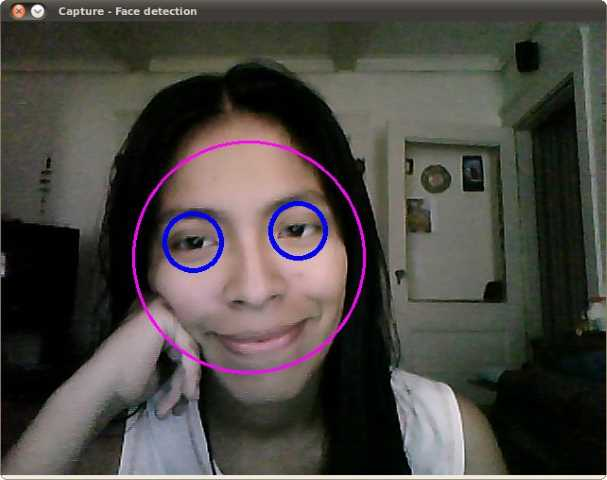
\includegraphics[width=.5\linewidth]{images/litreview/Cascade_Classifier_Tutorial_Result_Haar}
    \caption{Facial Recognition, image from \protect\footurl{https://docs.opencv.org/4.1.0/db/d28/tutorial_cascade_classifier.html}{OpenCV Cascade Classifier Tutorial}}
    \label{fig:facial}
\end{minipage}
\end{figure}

The main reasons to use OpenCV are because of its blazing speed, wide portability, and low RAM usage. It is entirely free to use, and what's more, it has frequently used and well maintained support forums, which is fantastic for when developers hit a brick wall in the applications. Further, they have annexed a set of experimental functions which extends the use cases of the library greatly.

On the other hand, reasons not to use OpenCV are that it does not provide the same ease of use when compared to other computer vision libraries such as MATLAB. In addition, the experimental modules come with the potential cost of bugs in various places, for instance, the Android pack for OpenCV with contribution modules fails to compile with their own build bots more often than it succeeds \citep{opencv-buildbot}.

\subsection{MATLAB}

Another software for computer vision is MATLAB, which is primarily designed for matrix manipulations, which makes it a good environment for data analysis and image processing. In contrast to OpenCV, MATLAB is commercial software that has more than 3 million users worldwide, and has been majorly profitable every year since its founding in 2017 \citep{matlabfacts}.

MATLAB can produce extremely stable software and functional codebase as a result of their dedicated team of professional developers, which in turn makes them popular among the masses. It can run highly parallelised code, making full use of GPUs and even clusters, which are large groups of computers that work together in a network to complete a task more efficiently. They also have the functionality to generate portable C code which can be used to develop Android and iOS applications. Further, the MATLAB GUI makes displaying output and debugging much more straightforward than its OpenCV counterpart.

Unfortunately, MATLAB requires a commercial licence to run, so to use it one must pay a fee or be fortunate enough to be under a company or campus-wide licence. Also, their libraries are well written, but not as cutting edge as OpenCV, so it fails to deliver on aspects of leading computer vision such as augmented reality.

\subsection{Summary}

After reviewing both OpenCV and MATLAB as candidates for the detection phase of this project, it is clear that OpenCV should be the method of choice, this is mostly because OpenCV is at the forefront of development for augmented reality. It is also natively portable because it is written in C++, as opposed to having to generate C code from MATLAB. The ability to parallelise MATLAB code is an excellent speedup feature; however, this project would not be able to use its full potential as the code will likely be running on a smartphone, which may be lacking in hardware.

%++++++++++++++++++++++++++++++++++++++++++++++++++++++++++++++++++++++++++++++++++
%++++++++++++++++++++++++++++++++++++++++++++++++++++++++++++++++++++++++++++++++++
%++++++++++++++++++++++++++++++++++++++++++++++++++++++++++++++++++++++++++++++++++

\section{Detection}

As mentioned previously, the detection of blocks and their poses is a vital stage of the project, and thus a key area of research. This section analyses various methods of both markerless and marker-based detection, and concludes by giving a recommendation into which method should be taken forward for design and implementation.

\subsection{Markerless Detection}\label{sec:markerless}

Markerless detection is a type of detection method used in augmented reality in which the system can detect objects in an environment without prior knowledge of that environment; this can be done by identifying features in an image and using that information to estimate the existence of a known object. A significant advantage of using markerless detection in this instance is that the \jenga{} blocks can remain unmodified and used out-of-the-box. As previously described, the best SDKs at the moment do not support detection of many objects at the same time, more specifically they would not be able to detect the poses of all 54 blocks in a tower. Therefore, it could be worth applying lower level image processing methods, such as the Hough-Lines Transform.

\subsubsection{Hough-Lines Transform}\label{subsec:hough}

The Hough-Lines transform \citep{houghpatent} is a popular feature extraction technique that can be used to identify lines that intersect many points in an image. It can also be expanded to find arbitrary objects, such as rectangles or circles. With \jenga{}, the transform can be used to detect edges of blocks which can later be used for tower reconstruction. The steps for finding lines with the hough transform are as follows:
\begin{enumerate}
    \item Load an image in grayscale
    \item Blur the image to reduce noise
    \item Apply Canny edge detection on the blurred, grayscale image
    \item Apply hough transform on the detected edges
\end{enumerate}

A simple program (\cref{code:houghpy}) was written to realize the potential of the transform with respect to block detection, the GUI for which can be seen in \cref{fig:houghscreenshot}, it shows an image for each stage of the hough transform process. Detected lines, drawn in red, can be seen traversing most edges of the tower pieces, but there are clearly edges that were missed. A serious advantage of this method is that it needs a minimal number of images, maybe even one, to get information about the tower pieces, it is therefore fast and non-intensive.

\begin{figure}[ht]
    \centering
    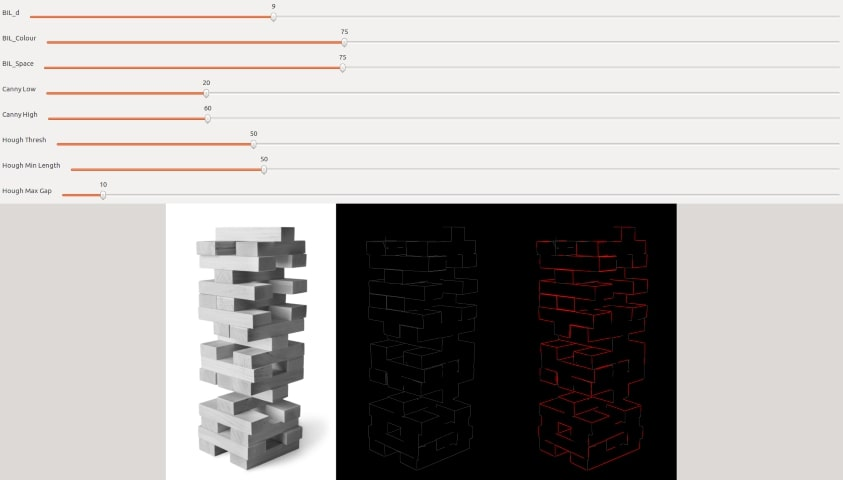
\includegraphics[width=.7\linewidth]{images/litreview/python-houghlines}
    \caption{Screenshot of hough.py program}
    \label{fig:houghscreenshot}
\end{figure}

This method would be disadvantageous to use because; it is difficult to detect every edge, meaning that a post hough-transform detection algorithm would need to be devised to find missing edges; poses would likely also be inaccurate; and the threshold values would need to be dynamic, as each environment has different lighting that would effect the methods used. Moreover, the transform has the potential to provide object tracking, but as the transform is low level, it would be hard to create a method of identifying an individual block, unlike the marker based detection methods that follow.

\subsection{Marker-Based Detection}\label{sec:markerbased}

Conversely to markerless detection, marker-based detection assumes knowledge of the environment with the use of fiducial markers. These markers are placed into the scene and are used as a point of reference to the camera, allowing for pose estimation. Two well-developed libraries to do this with are \nameandsecref{subsec:artoolkit} and \nameandsecref{subsec:aruco}, this section aims to cover the merits of both libraries and ultimately decide on which to implement in the system.

\subsubsection{ArToolKit}\label{subsec:artoolkit}

ARToolKit was one of the first libraries to make use of square markers for augmented reality applications. Its features include but are not limited to; the tracking of square markers, camera calibration, and plugins for Unity. With the kit, it is possible to get the pose of multiple markers in a single frame, which means that it would be able to detect all visible faces of blocks in a \jenga{} tower. This marker mapping feature makes it an ideal candidate for block detection.

\subsubsection{ArUco}\label{subsec:aruco}

\citet{aruco} is an alternate, newly developed library for marker-based detection. Since its inception, ArUco has been integrated with the contribution modules of OpenCV, making it a popular choice for marker detection. One of the benefits of using this library is the configurable dictionaries that aim to maximise inter-marker distance \citep{arucopaper}, hence reducing computation time when identifying markers. While the base code is written in C++, there are python and Java wrappers available, as well as cross platform support.

By itself, ArUco is unable to create a map of detected markers, however, \citet{markermapper} was created to solve this. \citet{markermapperpaper} demonstrate the effectiveness of using such a library, as it reduces pose ambiguity and can remember markers that are no longer visible to the camera. A drawback to using MarkerMapper is that if the map contains multiple components, that is if two or more maps of markers remain unconnected, the library results in a segmentation fault.

\citet{ucoslam} brings improvement to marker detection by adding functionality for simultaneous location and mapping (SLAM) of key points, and is shown to obtain better precision, robustness and speed than competing SLAM methods \citep{ucoslampaper}. This library fixes the aforementioned problem of multiple components because detected features are used to connect separate maps. It also provides an easy to understand GUI, and can be compiled for cross platform applications.

\begin{figure}[ht]
    \centering
    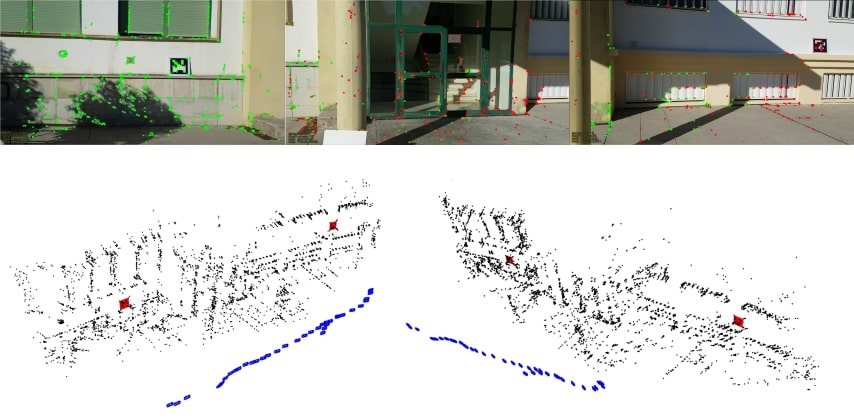
\includegraphics[width=.8\linewidth]{images/litreview/ucoslammapping}
    \caption{UcoSLAM mapping markers and key points. Image from \protect\citep{ucoslampaper}.}
    \label{fig:ucoslam}
\end{figure}

\subsection{Summary}\label{subsec:detectionsummary}

The research above shows that marker-based detection is favoured over markerless detection. Further, ARToolKit and MarkerMapper are able to produce similar results, but struggle with multiple map components. This could be an issue when detecting tower blocks because a camera may not be able to detect markers on two faces of the tower at the same time, resulting in unconnected marker poses. On the other hand, UcoSLAM would be able to detect other features of the tower, such as block corners, and use them to connect the faces of the tower. Although this means that UcoSLAM will be more compute heavy, it would be recommended to use UcoSLAM as the technology for block detection due to its obvious benefits.

%++++++++++++++++++++++++++++++++++++++++++++++++++++++++++++++++++++++
%++++++++++++++++++++++++++++++++++++++++++++++++++++++++++++++++++++++

\section{Reconstruction}\label{sec:reconstruction}

Next, to be able to analyse the structure, reconstruction must first take place, this can be done with modelling. A model is a computer-generated version of a real object which functions as if it were real. There are a multitude of methods which can be used to transform a real object into a model, these methods can be categorised in three ways:

\begin{itemize}
    \item \nameandsecref{subsec:partsbasedmodelling}, constructing a shape from a set of components
    \item \nameandsecref{subsec:voxelbasedmodelling}, constructing a shape from a set of volumetric elements
    \item \nameandsecref{subsec:viewbasedmodelling}, constructing a shape from an image or series of images
\end{itemize}

Whilst all of the methods described below are valid for constructing a model, they each have merits  and pitfalls, thus there is no 'silver bullet' approach to modelling. This section aims to provide research and critical evaluations of various methods, specifically relating to the modelling of a \jenga{} tower.
%+++++++++++++++++++++++++++++++++++++++++++++++++++++++++

\subsection{Parts-Based}\label{subsec:partsbasedmodelling}

\citet{2012probabilisticmodel} proposed a method which uses a set of shapes as training data, deconstructs them into a library of small parts, and then restructures those parts to make a set of new shapes. To do this, they used a probabilistic model to calculate which components fit together to form plausible combinations, which are defined by some optional high-level constraints. This approach proves useful in two applications; amplifying a shape database, and synthesising shapes based on high-level specifications.

An example of how this works is shown in \cref{fig:kchairs}. The model is trained on the set of chairs by taking them apart to get a set of the smallest functional components; backrest, legs, base. Next, a set of components from the training data is synthesised through the use of the probabilistic model. Finally, the components are scaled and placed together using the least-squares optimisation, thus a new shape has been synthesised.

% Chair figures
\begin{figure}[t]
\centering
\begin{subfigure}{.3\textwidth}
  \centering
  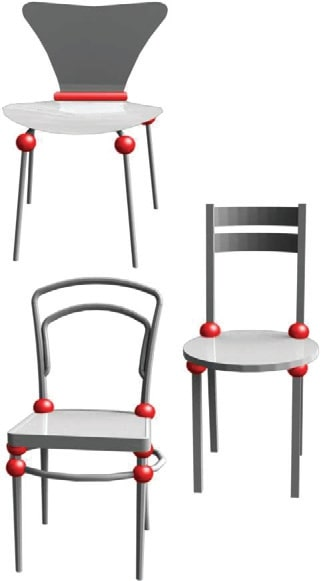
\includegraphics[width=.5\linewidth]{kalogerakis-chair-1}
  \caption{Source shapes}
  \label{fig:kchair1}
\end{subfigure}
\begin{subfigure}{.3\textwidth}
  \centering
  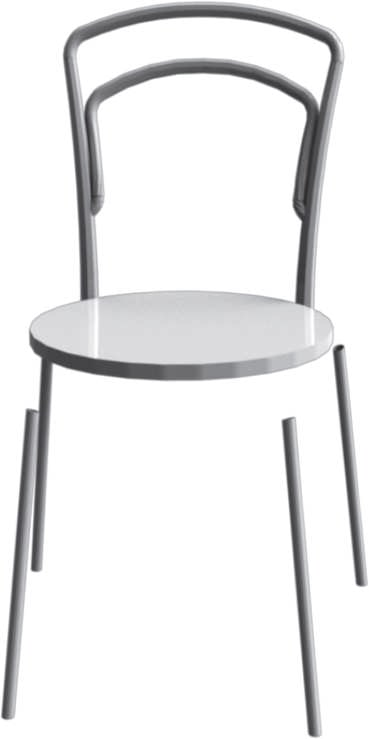
\includegraphics[width=.45\linewidth]{kalogerakis-chair-2}
  \caption{Unoptimised}
  \label{fig:kchair2}
\end{subfigure}
\begin{subfigure}{.3\textwidth}
  \centering
  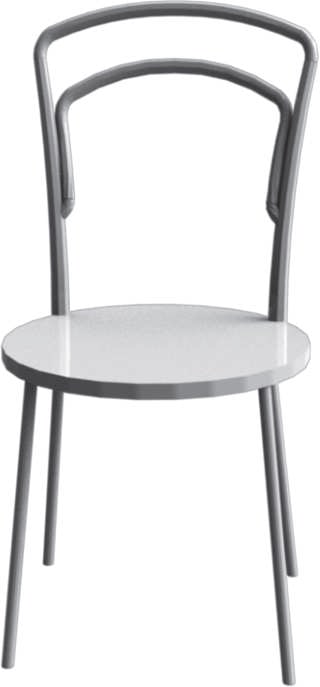
\includegraphics[width=.4\linewidth]{kalogerakis-chair-3}
  \caption{Optimised}
  \label{fig:kchair3}
\end{subfigure}
\caption{Optimising component placement. Images from \protect\citet{2012probabilisticmodel}.}
\label{fig:kchairs}
\end{figure}

A similar paper \citep{2015analysisandsynthesis} claims to have a superior approach to the synthesis of three-dimensional shapes. The method discussed in this paper is different than the one described above because it learns the geometry and deformation parameters of templates by itself, without the need to rely on pre-existing parts, which is favourable because it requires less human supervision. However, the learning is an approximation, and as such the quality of the produced shapes can be affected.

% The 3D-INN method
\begin{figure}[ht]
  \centering
  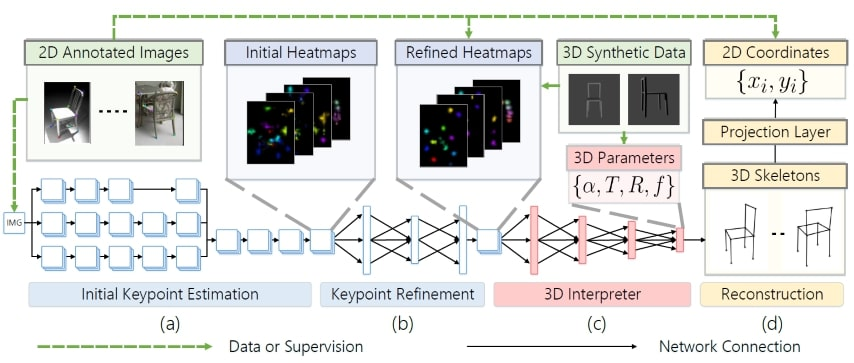
\includegraphics[width=.65\linewidth]{singleimageinterpreter}
  \caption{The 3D-INN method. Image from \protect\citet{2016singleimageinterpreter}.}
  \label{fig:3dinn}
\end{figure}

The 3D Interpreter Network method (\cref{fig:3dinn}), coined by \citet{2016singleimageinterpreter}, uses a trained framework to estimate a three-dimensional structure. The framework is trained using both synthetic 3D data and manually-annotated, real 2D images. Through the framework, they are able to extract a 3D skeleton which is treated as an abstract 3D representation. This method is part-based because the skeletons are synthesised using a predefined model for each object category, i.e. one model for all types of chair.

Finally, \citet{compoundscenesfromimages} proposed a method in which structures can be recovered from multiple silhouettes of a scene (\cref{fig:compoundscenes}). Their method works by using a library of predefined parts to find the simplest explanation of the shape of a scene. In their paper they describe that the method works for any scene, even if that scene does not contain any of the predefined parts, for example \cref{fig:eiffellego} shows a synthesised Lego construction of the Eiffel Tower. However, this method assumes that the images are taken from particular angles so that the model will not be constructed with holes when viewed from other angles.

% Lego part based modelling
\begin{figure}[ht]
  \centering
  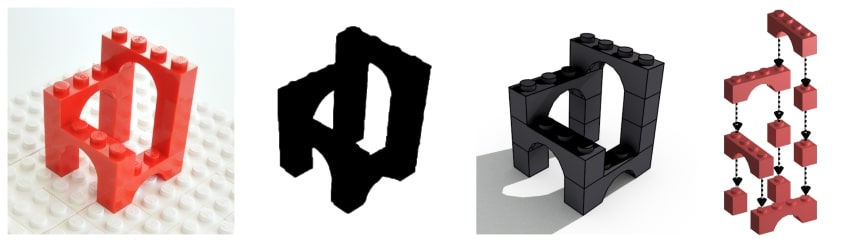
\includegraphics[width=.8\linewidth]{compound-scenes-demo}
  \caption{The part-based modelling of compound scenes from images method. Image from \protect\citet{compoundscenesfromimages}.}
  \label{fig:compoundscenes}
\end{figure}

% Lego part based modelling
\begin{figure}[th]
  \centering
  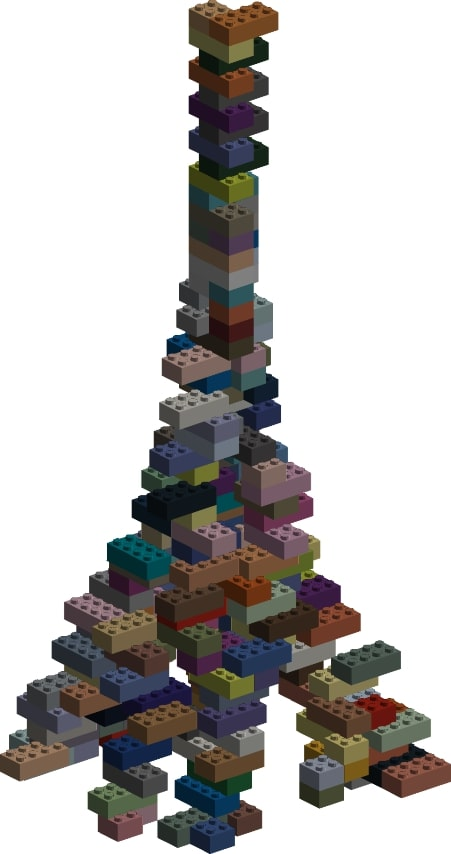
\includegraphics[height=4cm]{eiffel-tower-lego}
  \caption{Eiffel Tower constructed from Lego. Image from \protect\citet{compoundscenesfromimages}.}
  \label{fig:eiffellego}
\end{figure}

%+++++++++++++++++++++++++++++++++++++++++++++++++++++++++

\subsection{Voxel-Based}\label{subsec:voxelbasedmodelling}

A volumetric element, or voxel, represents a value in three-dimensional space akin to how a pixel represents a value in two-dimensional space. Large sets of voxels can be used to produce high quality and realistic renders of 3D shapes.

\citet{2016unsuplearning} outlined a method with which to construct a 3D shape from a 2D image using voxels. This method used end-to-end training solely from 2D images, which means they did not use any 3D annotated images, unlike a method touched on earlier \citep{2016singleimageinterpreter}. A large benefit of 2D image training in this manner is that it makes the approach entirely unsupervised. \citet{2016unsuplearning} also discuss using both volumes and meshes as elements to construct shapes, stating that volumes are flexible but introduce computational challenges, and that meshes are easier to work with, but can be restrictive in the range of shapes that they can capture.

Similarly, the 3D-GAN (3D Generative Adversarial Network) framework is learned without supervision, and has wide applications in 3D object recognition. \citet{2016problatent} state three benefits to their approach, namely the use of an adversarial criterion which allows the generator to capture object structure implicitly and thus the ability to synthesise high quality 3D shapes. Additionally they talk about the difficulty of modelling the space of 3D shapes, when compared to space of 2D objects, and how the various current approaches are promising but still produce objects with artefacts.

% The 3D-GAN method
\begin{figure}[th]
  \centering
  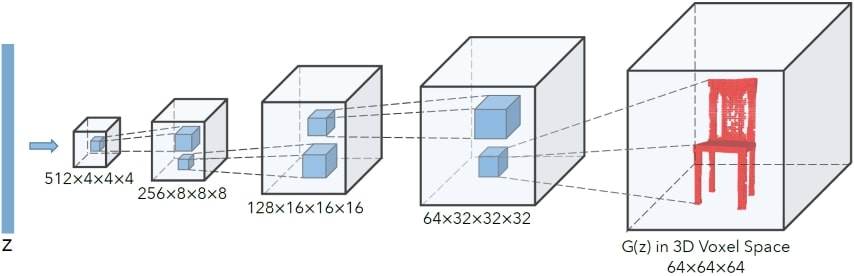
\includegraphics[width=.8\linewidth]{3D-GAN}
  \caption{The 3D-GAN method \protect\citep{2016problatent}.}
  \label{fig:3dgan}
\end{figure}

Another voxel-based modelling method, the TL-embedding network, consists of two components; an autoencoder, and a convolutional neural network (CNN). The network is multifunctional, but is focused on predicting 3D models from 2D images \citep{2016predictgenerativevector}. They specify that this approach demonstrates usefulness and versatility but the 3D representations may not incorporate the properties of the object they were synthesised from.

3D Shapenets \citep{20153dshapenets} is a model in which 3D shapes can be represented as a probability distribution of binary variables on a voxel grid. This model has the ability to recognise objects from 2.5D depth images, where a 2.5D image is effectively two-dimensional but can be perceived to have depth. \citet{20153dshapenets} learn their model using a Convolutional Deep Belief Network, though the use of a large dataset of 3D computer aided design models, and their experiments show that their representation shows significant performance improvements over previous state of the arts methods.

%+++++++++++++++++++++++++++++++++++++++++++++++++++++++++

\subsection{View-Based}\label{subsec:viewbasedmodelling}

Finally, models can be generated from a single or set of 2D images. 

\citet{2015convolutionalneuralnetworks} proposed a standard CNN architecture trained to recognise a 3D shape from a single view, with an accuracy 8\% higher than using state-of-the-art 3D shape descriptors, and their method increases in accuracy further when recognising a 3D shape from multiple views. Their method, shown in \cref{fig:multiview}, uses a view-pooling layer which is used to combine information from multiple views using their CNN architecture. What is interesting about this approach is that it can be used to recognise 3D objects even from a human sketch, as sketches can be less representative of the objects they are drawn from.

% Multiview approach
\begin{figure}[ht]
  \centering
  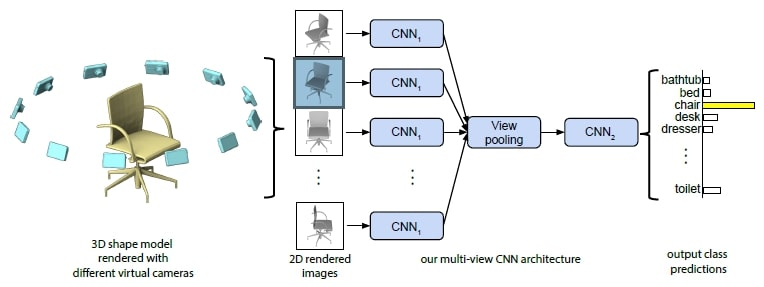
\includegraphics[width=.8\linewidth]{multiview}
  \caption{Multi-view CNN for 3D shape recognition. Image from \protect\citet{2015convolutionalneuralnetworks}.}
  \label{fig:multiview}
\end{figure}

In relation to the paper described above, \citet{2016volumetricmultiview} performed extensive experiments on the classification accuracy of state-of-the-art 3D volumetric CNN and multi-view CNN. They found that multi-view CNN far outperformed volumetric CNN, as shown in \cref{fig:volvsviewcnn}.

% Volumetric vs multiview
\begin{figure}[th]
  \centering
  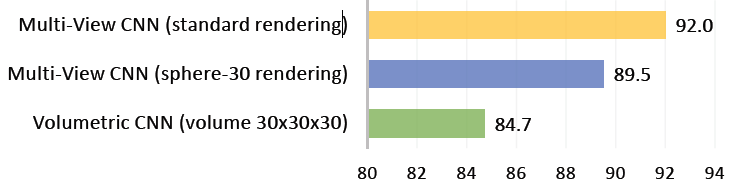
\includegraphics[width=.8\linewidth]{volumetric-vs-multiview-cnn}
  \caption{Analysis of state-of-the-art 3D Volumetric CNN versus Multi-View CNN. Image from \protect\citet{2016volumetricmultiview}.}
  \label{fig:volvsviewcnn}
\end{figure}

%++++++++++++++++++++++++++++++++++++++++++++++++++++++++++++++++++++++
%++++++++++++++++++++++++++++++++++++++++++++++++++++++++++++++++++++++

\subsection{Summary}\label{sec:categoriessummary}

The most suitable category for modelling a \jenga{} tower in this project is part-based modelling, this is mainly due to the ease of representing a tower as a combination of \jenga{} blocks. In the part-based modelling papers that were expanded in this section, most used an extensive library of 3D objects, however when modelling a \jenga{} tower only one 3D object is needed, as it can be assumed that all blocks have the same width, height and depth. Of course, the blocks may have slight variations in shape, but this can be mostly ignored for the scope of this project. A considerable benefit of using part-based modelling is that it encapsulates the reconstruction stage, and so the models created can be used directly and without further work, in the analysis stage.

In comparison, voxel-based methods can be used to synthesise high quality 3D models, but these models are likely to contain artefacts. Artefacts would be disadvantageous when creating a model of a \jenga{} tower because they would affect its structural integrity, for example a block may be generated with rough or noisy edges meaning that the blocks above it will not sit evenly on top and cause instability. So artefacts may cause an invalid representation of the real tower, making voxel-based methods less suitable to \jenga{} tower modelling.

View-based modelling has a suitability higher than that of voxel-based methods, this is because view-based methods produce models in a lower amount of time and with higher accuracy. The time it takes to model a \jenga{} tower is important because the end product needs to be able to extract structure in real-time, or close to real-time, so that the process is not painful for the user. However, view-based methods are less suitable than part-based methods because extra work needs to be done on the models after their generation to allow structural analysis to be performed.

%++++++++++++++++++++++++++++++++++++++++++++++++++++++++++++++++++++++
%++++++++++++++++++++++++++++++++++++++++++++++++++++++++++++++++++++++



%++++++++++++++++++++++++++++++++++++++++++++++++++++++++++++++++++++++++++++++++++
%++++++++++++++++++++++++++++++++++++++++++++++++++++++++++++++++++++++++++++++++++
%++++++++++++++++++++++++++++++++++++++++++++++++++++++++++++++++++++++++++++++++++

\section{Analysis}\label{sec:structuralanalysis}

The main objective in \jenga{} is to remove a block from the tower and place it on top, in such a way that the tower remains structurally intact. Choosing which block to remove is a difficult task, as the analysis relies heavily on the physics of structural engineering. This section will provide a background in a few types of structural analysis, namely \nameandsecref{subsec:rulebased}, \nameandsecref{subsec:physicssimulation}, and \nameandsecref{subsec:machinelearning}, it will then give a summary of what was researched and identify some key points for consideration later on in the project.

%++++++++++++++++++++++++++++++++++++++++++++++++++++++++++++++++++++++
%++++++++++++++++++++++++++++++++++++++++++++++++++++++++++++++++++++++

\subsection{Rule-Based Analysis}\label{subsec:rulebased}

\citet{jengaanalysis} researched into the translations and rotations that can be performed on \jenga{} blocks in a tower to find out which moves are safe from disturbing other blocks. He concluded that the movement that resulted in the least disturbance to the tower, for a centre block, was one which included no rotation, and only translation in a single direction; perpendicular to the face of the tower that the block is being removed from.

In his paper, he also mentions the most significant factor that complicates the game is the variability of the game pieces, a fact confirmed by \jenga{}'s creator \citep{jengacreator}, this is because smaller blocks can become free-floating, and larger blocks can become load bearing. When rebuilding the tower in a virtual space, it would be difficult to counteract this problem unless the blocks had their dimensions measured individually, which is a time sink and reduces the usability of the system.

\begin{figure}[ht]
    \centering
    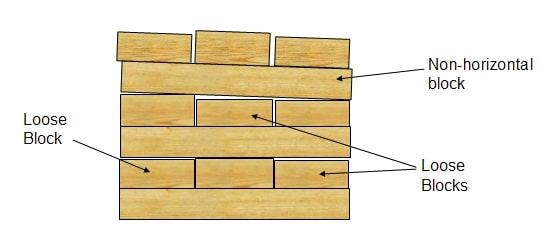
\includegraphics[width=.8\linewidth]{images/litreview/jenga-different-sizes}
    \caption{A side view of a \jenga{} tower \protect\citep{south2003real}}
    \label{fig:jengasizes}
\end{figure}

In another light, \citet{jengarobot} created a robot capable of playing \jenga{} for a tower of up to 9 layers, although the robot wasn't able to place the pieces back on top of the tower. His paper was full of useful information about the block extraction process, including the differences between side and centre blocks. It was established that the centre pieces were easier to remove, but subsequent moves on that layer would result in collapse, in contrast, both edge pieces could be removed on one level with minimal affect on the tower stability.

In summary, it is plausible to have a set of rules accurate enough for rule-based analysis, yet it may not be the most effective way to analyse the tower. This analysis method only provides simple rules, and is missing more advanced constraints such as friction and weight distribution.

%++++++++++++++++++++++++++++++++++++++++++++++++++++++++++++++++++++++
%++++++++++++++++++++++++++++++++++++++++++++++++++++++++++++++++++++++

\subsection{Physics Simulation}\label{subsec:physicssimulation}

This section will review some of the many \jenga{} simulators already exist, and discuss their uses in this project.

\subsubsection{\protect\possessivecite{github-Physijs} Jenga Physijs}

A fantastic simulator using the Physijs implementation of ammo.js, a Bullet physics engine. On opening the simulator, the tower visibly sways a small amount, indicating that the pieces all have pre-allocated positions in the world, and when gravity acts on the tower, it moves slightly until it reaches equilibrium. On moving the blocks, the inter-block contact feels slippery, as if the friction was not quite calibrated to real-world \jenga{} blocks. The physics of the tower seems to accurately represent what would happen with a real tower in the same state.

There was however a major problem found during testing; occasionally when moving a piece, it would shoot off at high speed, which is unrealistic. It is possible that the simulator misinterpreting mouse events could cause this, but could also be due to the weight of the tower forcing the block out, either way this kind of bug is game-breaking.

The source code is available on GitHub so it would be possible to fork the project for use in this paper, but the game-breaking bug would have to be addressed, and functions added for importing a tower state.

\begin{figure}[ht]
\begin{minipage}{0.45\textwidth}
    \centering
    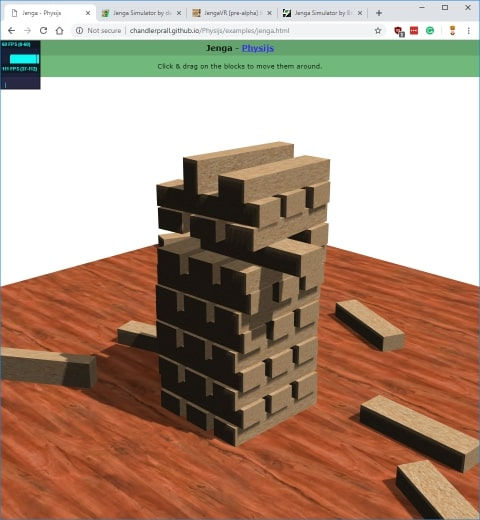
\includegraphics[width=.8\linewidth]{images/litreview/jenga-2}
    \caption{An instance of Jenga Physijs \protect\citep{github-Physijs}}
    \label{fig:simulator1}
\end{minipage}\hfill
\begin{minipage}{0.45\textwidth}
    \centering
    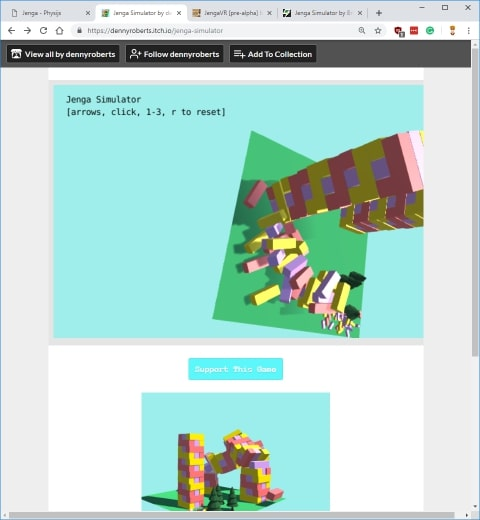
\includegraphics[width=.8\linewidth]{images/litreview/jenga-1}
    \caption{An instance of Jenga-Simulator \protect\citep{itchjenagasimdennisroberts}}
    \label{fig:simulator2}
\end{minipage}
\end{figure}

\subsubsection{\protect\possessivecite{itchjenagasimdennisroberts} Jenga-Simulator}

This simulator is built in Unity for use on the web; it has a distinctive multicoloured theme which makes it easy to distinguish between the tower pieces. On startup, the game drops a set of blocks from the sky onto a small platform, where they settle to form towers, immediately it can be seen that this sequence would fail to work with an imported tower of any other state than the starting state.

It also works by clicking, instead of dragging, which makes for a rather odd experience. As a result of only allowing clicks, movements are restricted to translations, which meant that removing by rotation was out of the question. Another aspect that stood out was that the whole scene moved when clicking, and therefore the whole tower was affected regardless of whether a block could be removed successfully.

In terms of friction though, this simulator stood above \possessivecite{github-Physijs} because it did not feel slippery, but more like real movements of \jenga{} blocks.

\subsubsection{\protect\possessivecite{itchjengasimben} JengaVR}

JengaVR is only available in virtual reality, and due to limited access to VR headsets, first-hand testing could not be done. Nonetheless, there are a couple of videos on the web in which this game was played, and as such this review is completed from watching the game second-hand.

It was nice to see that the in-game blocks had the same texture as real \jenga{} blocks, as it allowed for a more immersive experience. Picking out pieces of the tower looked intuitive, as the player can use hand-held controllers similar to how they would play outside of the virtual world.

Further, the tower seemed shaky at times and swayed at others. At one point, a block was edging inside of another, meaning that the collision detection was not as accurate as it should be. Also, the tower looked like it should have fallen over in a couple of states, but this was maybe prevented by a higher amount of friction in the game engine.

\begin{figure}[ht]
    \begin{minipage}{0.45\textwidth}
        \centering
        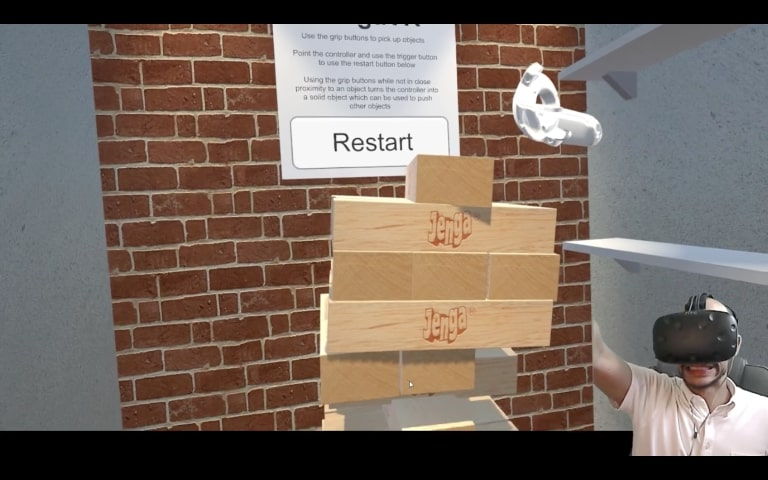
\includegraphics[width=.9\linewidth]{images/litreview/jenga-3}
        \caption{Screencap from the JengaVR trailer \protect\citep{github-Physijs}}
        \label{fig:simulator3}
    \end{minipage}\hfill
    \begin{minipage}{0.45\textwidth}
        \centering
        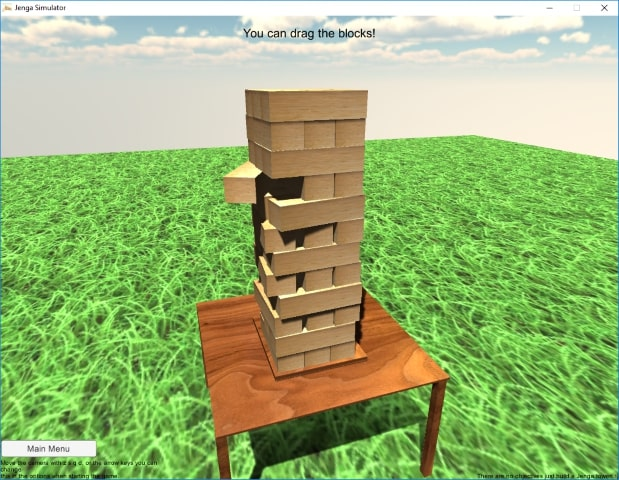
\includegraphics[width=.9\linewidth]{images/litreview/jenga-4}
        \caption{An instance of Jenga-Simulator \protect\citep{gamejoltjengasim}}
        \label{fig:simulator4}
    \end{minipage}
\end{figure}

\subsubsection{\protect\possessivecite{gamejoltjengasim} Jenga-Simulator}

In this Windows based Jenga-Simulator, a \jenga{} tower sits on top of a table in a semi-realistic world, for the user to play with. Blocks can be dragged with the mouse, and the camera moves on a plane on one side of the tower, if any of the blocks fall, the game restarts.

Removing pieces from the tower in this game proved more difficult than any of the other simulators, perhaps due to the high amount of friction, which may have been avoided by creating slight variations in the block dimensions, as it allows for free-standing pieces.

This game was the most fun to play, but it did not feel realistic, which was partly due to the blocks not being of the standard \jenga{} dimensions, and also because of the difficulty in removing the pieces.

\subsubsection{Summary}

All of the above were made to be played as games, not realistic simulators, so during development there was bound to be decisions which opted for enjoyability over realism. One of these decisions was to create blocks that did not accurately represent the size of \jenga{} blocks. Despite this, there is still a lot that can be learned from these projects.

Firstly, creating blocks of randomly varying sizes would fix some of the issues observed, but the same could not be said for the system proposed in this document.  If the tower were to be built with varying sizes, they would have to be the real sizes of the blocks, not random; otherwise the simulation would not accurately represent the real tower.

A common issue was that the friction was either too high, causing difficulty in removal, or too low, causing a slippery feel to the game. It would be beneficial to test out several settings of friction during the development of this project, to ensure realism is achieved.

%++++++++++++++++++++++++++++++++++++++++++++++++++++++++++++++++++++++
%++++++++++++++++++++++++++++++++++++++++++++++++++++++++++++++++++++++

\subsection{Machine Learning}\label{subsec:machinelearning}

Machine learning, a term coined by \citet{machinelearning}, is the study of computer algorithms which rely on patterns and inference to perform specific tasks. The taxonomy of these algorithms include; supervised learning, where the algorithm learns with labels given by human input, unsupervised learning, where the algorithm learns without human input, and reinforcement learning, where the algorithm learns a policy of how to act given an observation of the world, i.e. learn from its mistakes \citep{machinelearningtypes}.

In essence, machine learning is used for tasks that are too complex for developers to code a solution for themselves, and is therefore useful in many areas; applications range from autonomous helicopter aerobatics \citet{autonomoushelicopter}, to the early detection of heart failure \citep{machinelearningheart}. There are numerous factors involved with the physics of a \jenga{} tower, making it difficult to accurately assess, this section discusses whether it would be appropriate to involve machine learning to aid in the analysis.

\subsubsection{Supervised}

Supervised learning is maybe the most popular paradigm for machine learning; it is synonymous with giving an algorithm labelled data which are then used to predict the classification of unseen data. This project could make use of supervised learning techniques by generating a set of training data which would include a great many variations of tower states, and then labelling each state with either stable, or unstable. During system runtime, if the algorithm comes across a tower state that is not included in the training data, it would then be able to give a prediction on the classification of tower state.

Although popular, this type of machine learning would require a lot of time spent training, as the human trainer would need to manually classify each state, and so would not be an ideal choice of method for this project.

\begin{figure}[ht]
\begin{minipage}{\textwidth}
    \centering
    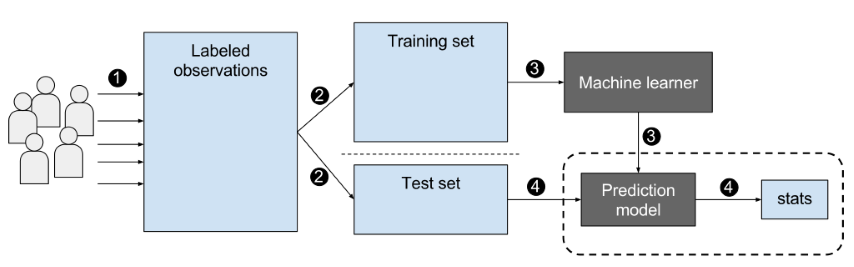
\includegraphics[width=.8\linewidth]{images/litreview/Supervised_machine_learning_in_a_nutshell}
    \caption{Supervised learning from  \protect\footurl{https://blogs.nvidia.com/blog/2018/08/02/supervised-unsupervised-learning/}{Nvidia Blogs}}
    \label{fig:supervisedlearning}
\end{minipage}
\end{figure}

\subsubsection{Unsupervised}

On the other hand, unsupervised learning is a data-driven approach that does not require labelling; it is instead fed data and tries to discover the underlying structure of that data. As a result of the learning being unsupervised, there is no way to determine what the outcomes would be, nor how accurate they are, and as such, this approach is not well suited to classification problems. 

In the case of this project, the data would again be a set of many variations of tower states, but the results could be wildly different the supervised approach. It would be interesting to see what these would be, but probably falls out of the scope of this project.

\subsubsection{Reinforcement}

Finally, reinforcement learning is an machine learning approach akin to Pavlov's dog \citep{pavlovdog}, in which the behaviour conditioning of dogs were recorded in response to varying stimuli. With respect to machine learning, this technique allows an algorithm to learn from mistakes, by providing it with positive and negative signals after performing a task.

\begin{figure}[ht]
    \centering
    \begin{tikzcd}
        Perception \ar[r] & Action \ar[r] & Reward \ar[ll,bend left,"repeat"]
    \end{tikzcd}
    \caption{Reinforcement learning pipeline}
\end{figure}

This approach would encompass giving the algorithm full reign of a \jenga{} simulator, meaning it would have the ability to move blocks, just like a human would in the real world. First, the algorithm would choose a block, and attempt to remove it, if the removal causes the tower to fall over then it would record the result as a negative stimulus, otherwise a positive result would be recorded. Then, the tower would be rebuilt and the process would repeat itself many times over, with the algorithm learning with each iteration.

\subsubsection{Summary}

In summary, given a trained algorithm, the system would be able to analyse the structural integrity of a \jenga{} tower, and give the user a prediction of the removal feasibility of each block. The preferred method described above is reinforcement learning, this is because of it's ability to learn from its mistakes, and because it is a more autonomous technique than supervised learning, which would require lots of human input. In contrast, unsupervised learning would not be ideal for this project as the results would be unpredictable.

%++++++++++++++++++++++++++++++++++++++++++++++++++++++++++++++++++++++++++++++++++
%++++++++++++++++++++++++++++++++++++++++++++++++++++++++++++++++++++++++++++++++++
%++++++++++++++++++++++++++++++++++++++++++++++++++++++++++++++++++++++++++++++++++

\section{Visualisation}

The last area to be researched for this project is the presentation stage. The topics covered in this background study comprises of visual display techniques, including augmented reality, and graphical user interfaces (GUIs).

%++++++++++++++++++++++++++++++++++++++++++++++++++++++++++++++++++++++
%++++++++++++++++++++++++++++++++++++++++++++++++++++++++++++++++++++++

\subsection{Head-Worn Displays}

Head-worn displays boast a more immersive experience than AR on smartphones, yet they can be considerably more expensive. Currently, there are a wide variety of head-worn displays on the market, some of which are reviewed below with relation to this project.

\subsubsection{Microsoft HoloLens 2}
The HoloLens 2 \citep{hololens2} is the latest in the line of HoloLens headsets, with improvements over its predecessors such as a wider field of view, eye tracking sensors, and being lighter in weight. Although, with a price tag of \$3,500, this device is not aimed towards the general public, but mostly at businesses that could see improvements through the use of AR, such as factory workers. A consequence of the cost to purchase the HoloLens is that it would be infeasible to use in an undergraduate project.

\subsubsection{North Focals}
More realistically priced, the \citet{northfocals} are a pair of AR glasses that cost around \$599. They look like standard, non-technological glasses, but have much functionality built in, like text messages, music and maps. While aesthetically pleasing and custom built, these glasses seem to be great for the everyday consumer, when it comes to augmented reality for gaming, they fail to deliver, due to their low specification hardware.

\subsubsection{Intel Vaunt}
HoloLens and North Focals both use a screen display method, Intel's Vaunt breaks this pattern by using laser projection; the glasses work by reflecting a laser beam into the eyeball, and onto the retina. The laser used is of class one, which means it is very low powered, and will not cause harm to the eye. Unfortunately, the Vaunt is officially no longer being developed \citep{intelvaunt}, so it would not be possible to use it in this project.

\subsubsection{Magic Leap One}
The \href{https://www.magicleap.com/magic-leap-one}{Magic Leap} (\citeyear{magicleap}) is also separate from on-screen AR display, as it projects a digital light field into the user's eye \citep{redditmagicleap}, which is apparently the only safe way forward for authentic replication of visual reality. It requires the user to carry around a small Lightpack which performs all of the computations for displaying AR with the goggles, while retaining its mobility. It also has a controller, which allows it to be used for games, so in that respect, it would be suitable for use in this project. But as an emerging technology, the Magic Leap One is not yet available to consumers, but people in a few United States cities do have access to the device in a development capacity.

\begin{figure}[ht]
\begin{minipage}{\textwidth}
\begin{minipage}{0.5\textwidth}
    \centering
    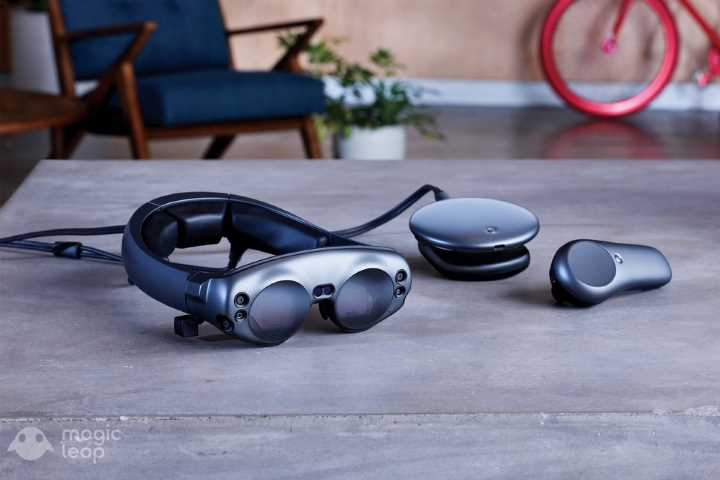
\includegraphics[width=0.9\textwidth]{images/litreview/magicleap}
    \label{fig:magicleap}
\end{minipage}\hfill
\begin{minipage}{0.5\textwidth}
    \centering
    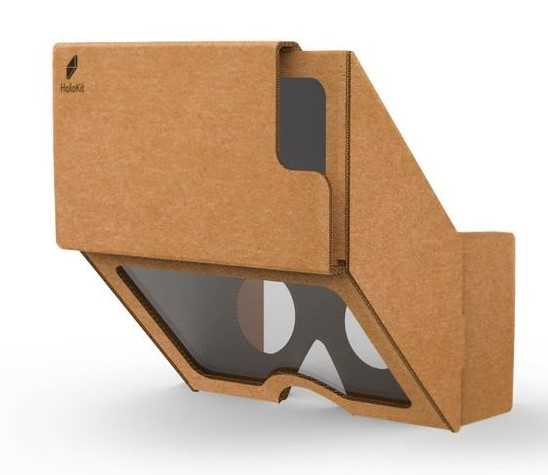
\includegraphics[width=0.7\textwidth]{images/litreview/holokit}
    \label{fig:holokit}
\end{minipage}
\caption{The \protect\footurl{https://www.magicleap.com/magic-leap-one}{Magic Leap One} (left) and the \protect\footurl{https://holokit.io}{HoloKit} (right)}
\end{minipage}
\end{figure}


\subsubsection{Lenovo Mirage}
Down in the low end of AR headsets sits the \href{https://www.lenovo.com/gb/en/jedichallenges/}{Lenovo Mirage} (\citeyear{jedi}), at just \pounds89.99, providing an experience like no other around today. This device is built solely for AR gaming, specifically for Star Wars, a popular film and tv franchise; it offers lightsaber duels, ship battles, and other strategic games, all played in augmented reality. Also, the headset requires a smartphone, which is used as a display device; meaning it would be useful in this project as any smartphone app can be used.

\subsubsection{HoloKit}
Related to the Lenovo Mirage, the \href{https://holokit.io}{HoloKit} (\citeyear{holokit}) requires a smartphone to function. It is made from cardboard and works by having the phone reflect its display onto a mirror next to the user's eyes. Moreover, it is maybe the cheapest AR headset available today, owing to its minimalist design. The HoloKit software development kit (SDK) is available on GitHub and uses the Unity game engine to create applications.

\subsubsection{Summary}
It is exciting to use augmented head-worn displays because they use cutting edge technologies, meaning that many of the experiences they offer have never been seen before.  However, this also brings drawbacks, namely the high prices and low availability. A common theme among the above devices is the inability to provide gaming in the experience; this is because some of the glasses are not designed for such functions. They also need to have high mobility, as they are expected to be used in a diversity of environments, and need to be as efficient as possible, leading to lower power consumption and consequently lower battery sizes. 

The most appropriate displays identified are the Lenovo Mirage and HoloKit because of their incorporation of smartphones, meaning they can display any mobile application, at a low cost. Although, if considering this route it would be less expensive to not use a head-worn display at all, with the downside of having to hold the phone with hands.

All things considered, head-worn displays are not yet quite as developed, economical, or featureful as would be needed for a project of this description, and so it would be recommended not to use headsets.

%+++++++++++++++++++++++++++++++++++++++++++++++++++++++++

\subsection{Software Development Kits}

In order to develop applications in augmented reality, software development kits (SDKs) must be used. AR SDKs are bundles of useful functions that allow developers to interact with the environment through various computer vision techniques, which saves time during application development because it prevents reinventing the wheel. This section shows the research completed into four of the significant AR SDKs prevalent today that work with modern smartphones; Vuforia, ARKit, ARCore, and ARToolkit.

\subsubsection{Vuforia}
\href{https://www.ptc.com/en/products/augmented-reality}{Vuforia} (\citeyear{vuforia}) is an SDK which provides recognition for objects, text and environment. It is marketed mainly for industrial use, including solutions for manufacturing, reducing service costs, and sales. Also, it prides itself with a powerful object scanner, which allows the user to scan and create real object targets for rigid objects that can fit on a tabletop.

\begin{figure}[ht]
\begin{minipage}{\textwidth}
    \centering
    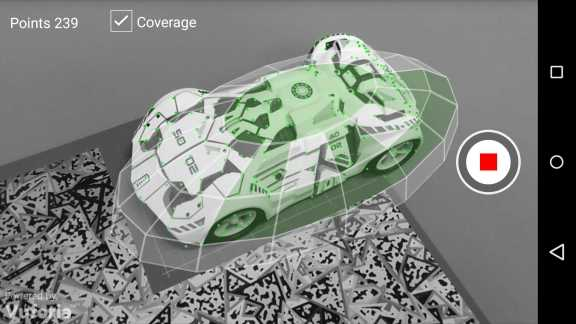
\includegraphics[width=0.6\textwidth]{images/litreview/vuforiaobject}
    \caption{Object scanning in Vuforia, image from \protect\footurl{https://library.vuforia.com/articles/Training/Vuforia-Object-Scanner-Users-Guide}{Vuforia Users Guide}}
    \label{fig:vuforia}
\end{minipage}
\end{figure}

This scanner could be used to create a virtual \jenga{} block object, with high precision, and later used for augmented display. Alas, the engine only supports tracking of up to two objects at a time, rendering this solution unworthy, at least while the object tracking limit remains this low.

\subsubsection{ARKit}
Apple Inc. purchased the \citeauthor{arkit} in 2015, and have continued development since then, so far providing features such like; the TrueDepth camera system, which combines several sensors to get an accurate understanding of depth in images; visual inertial odometry, where the pose of a camera can be estimated using images of its environment; ambient lighting estimation, which it uses to update the colours of virtual objects based on its surrounding light.

ARKit, as with most Apple products, is contained within the Apple ecosystem, which means that the SDK is only available on a few select smartphones produced by the company. As a direct result from this, ARKit was not able to be used in this project on account of limited resources.

\subsubsection{ARCore}\label{sec:arcore}
Similar to ARKit is Google's \citet{arcore}, which shares many of its features, and adds motion tracking and more advanced environmental understanding, allowing for augmented objects to be seemingly connected to real-world objects, rather than just superimposed. In contrast to ARKit, ARCore is available on a plethora of devices, including some on iOS.

Currently, the SDK can track objects, but this is implemented to estimate the camera pose, so it would be ineffective for predicting individual block poses. However, a solution in which the tower is tracked as a single rigid object may be viable with this technology.

\begin{figure}[ht]
\begin{minipage}{\textwidth}
    \centering
    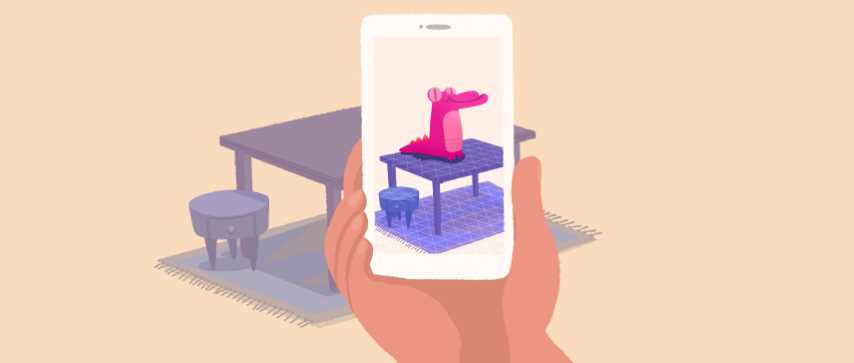
\includegraphics[width=0.8\textwidth]{images/litreview/EnvUnderstanding}
    \caption{Environmental understanding in ARCore, from \protect\footurl{https://developers.google.com/ar/discover/concepts}{Google Discover Concepts}}
    \label{fig:arcoreenv}
\end{minipage}
\end{figure}

\subsubsection{ARToolKit}
\citet{artoolkitandroid} reviewed the development process of creating an augmented reality application for Android devices using the \citet{artoolkit} SDK, an open source library that implements the logic necessary for AR applications. In the report she says that the SDK works with ordinary phones and webcams, which is unlike the kits reviewed above, as they all require reasonably well-powered smartphones. A key feature in ARToolKit is marker tracking and pose estimation, this allows the developer to track multiple objects at a time, provided they have markers attached.

\subsubsection{Summary}
The software development kits described above are all at the forefront of AR technology today, and so represent the best functionality that AR has to offer. After review, it is clear that tracking objects, such as \jenga{} blocks, would be difficult, unless marker based AR is used. Otherwise, it may prove worthwhile to track the tower as a single structure, and augment information directly onto that, but this has its own drawbacks, for instance the pieces would not be able to be tracked when being removed from the structure. The next sections delve more into this discussion by comparing markerless and marker based AR.

\subsection{Interfacing}

Paired with an augmented display, a graphical user interface (GUI) is key to providing the user with a pleasant experience. Much research has been completed in this topic, from this research, the section below gives some insight into what it takes to design an efficient and user-friendly interface.

\possessivecite{guirooms} paper on designing user interfaces is an example of early work in the field; it focuses on reducing space contention in a window-based GUI by using a window management concept called Rooms. Although this paper was written a couple of decades before the rise of smartphones and AR, there are still some relevant points to be considered. One of which is to avoid the ``electronic messy-desk problem'', where too many items are displayed on a screen, leading to a reduction in workspace efficiency and performance.

More recently, \citet{guienergyefficiency} showed that significant improvements to GUIs can be made by employing energy efficient design techniques. A survey they conducted found several intuitions into GUI use, such as; users find small buttons annoying, users prefer interfaces that are easy to learn and allow them to work faster over good-looking interfaces, as well as liking features which display progress is being made, such like an hourglass.

Furthermore, usability studies show great promise in the design of user-friendly mobile interfaces. \possessivecite{guiusabilityreview} review into the area concluded that some of the main qualities in the design of these interfaces are limited screen size, lack of physical response and high demand for visual attention. It is, therefore, necessary to take into account these areas when designing the interface for the proposed solution in this document.

A current interface can be seen when using the IMDb smartphone app (\cref{fig:imdb}), which uses many features common to applications today. The app keeps the amount of displayed text minimal, so as to rapidly identify areas of importance to the user, such as headings. It also uses large images, this is because images are more interesting than text and serve to capture the users attention. In addition, IMDb has uses a scrolling interface which allows the user to display more content when they have finished consuming the current content, this is useful when an app has more information than it can comfortably fit on one screen. Another point of reference is the tab bar layout at the top of the app, which makes it clear which page the user is currently viewing, and allows the user to switch between pages with ease.

\begin{figure}[ht]
\begin{minipage}{\textwidth}
    \centering
    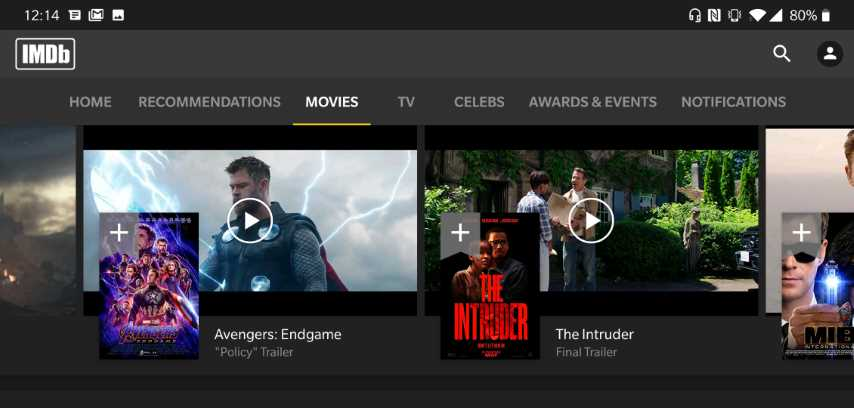
\includegraphics[width=\textwidth]{images/litreview/imdb-screenshot}
    \caption{A modern smartphone interface, from the \protect\footurl{https://play.google.com/store/apps/details?id=com.imdb.mobile&hl=en_GB}{IMDb Android Application}}
    \label{fig:imdb}
\end{minipage}
\end{figure}

%++++++++++++++++++++++++++++++++++++++++++++++++++++++++++++++++++++++++++++++++++
%++++++++++++++++++++++++++++++++++++++++++++++++++++++++++++++++++++++++++++++++++
%++++++++++++++++++++++++++++++++++++++++++++++++++++++++++++++++++++++++++++++++++

\subsubsection{}

This chapter has researched and discussed various literature and technology surrounding the project scope. Findings from this background study will influence the decisions made later on in the project, including being the main source for the capture of requirements, which will follow.

%++++++++++++++++++++++++++++++++++++++++++++++++++++++++++++++++++++++++++++++++++
%++++++++++++++++++++++++++++++++++++++++++++++++++++++++++++++++++++++++++++++++++
%++++++++++++++++++++++++++++++++++++++++++++++++++++++++++++++++++++++++++++++++++
